\documentclass{article}
\usepackage{inputenc,fullpage,enumitem,amsmath,amssymb,graphicx}
\usepackage{hyperref}

\title{Cloud computing Homework 1}
\author{Hao Yu}
\date{October 15 2021}

\begin{document}

\maketitle

\begin{abstract}
This assignment is an RPC experiment, divided into the following parts, RPC principle, experimental environment, experimental details, source code and conclusion.
\end{abstract}

\section{RPC principle}\label{sec:rpc-principle}
\begin{enumerate}[label=(\alph*)]
  \item {
    Remote procedure call (RPC) is a technology used to build distributed, client-server based applications.
    It is based on extending the conventional local procedure calling so that the called procedure need not exist in the same address space as the calling procedure.
  }
  \item {
    Figure~\ref{fig:rpc} is the model of remote procedure call.
    \begin{figure}[htp]
        \centering
        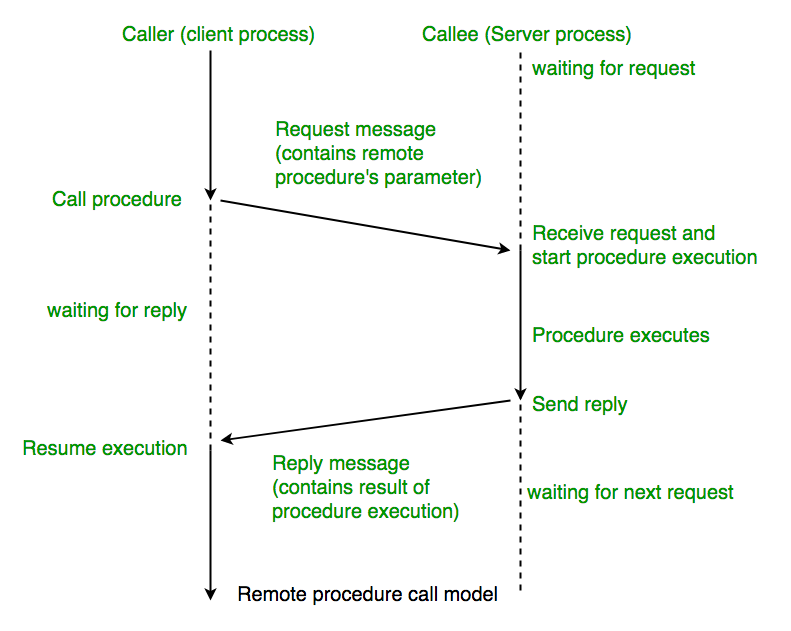
\includegraphics[width=10cm]{rpc}
        \caption{Remote procedure call model}
        \label{fig:rpc}
    \end{figure}
  }
\end{enumerate}

\section{Experimental environment}\label{sec:experimental-environment}
\begin{enumerate}[label=(\alph*)]
  \item {
    The programming language used in the experiment program is Python, and the version is 3.7.
  }
  \item {
    The RPC package used in the experimental program is RPyC. RPyC (pronounced like are-pie-see), or Remote Python Call, is a transparent library for symmetrical remote procedure calls, clustering, and distributed-computing. RPyC makes use of object-proxying, a technique that employs python’s dynamic nature, to overcome the physical boundaries between processes and computers, so that remote objects can be manipulated as if they were local.
  }
  \item {
    The client is deployed on macOS. Figure~\ref{fig:client_sysinfo} shows the system information.
    \begin{figure}[htp]
        \centering
        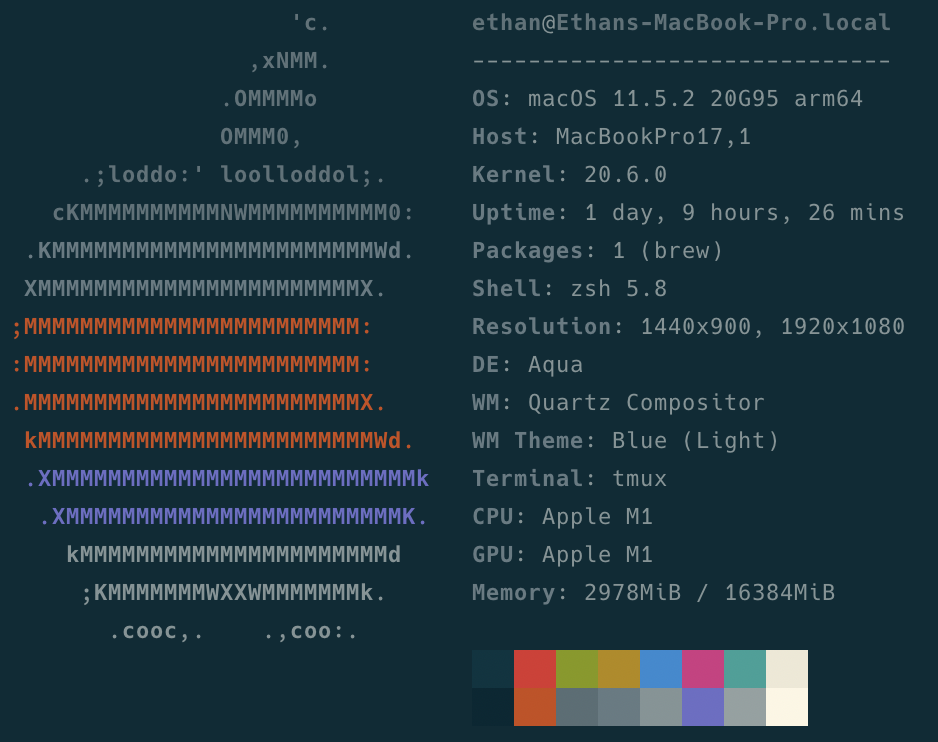
\includegraphics[width=10cm]{client_sysinfo}
        \caption{Client system information}
        \label{fig:client_sysinfo}
    \end{figure}
  }
  \item {
    The server is deployed in the docker container of an Azure server in the US. Figure~\ref{fig:server_sysinfo} shows the system information.
    \begin{figure}[htp]
        \centering
        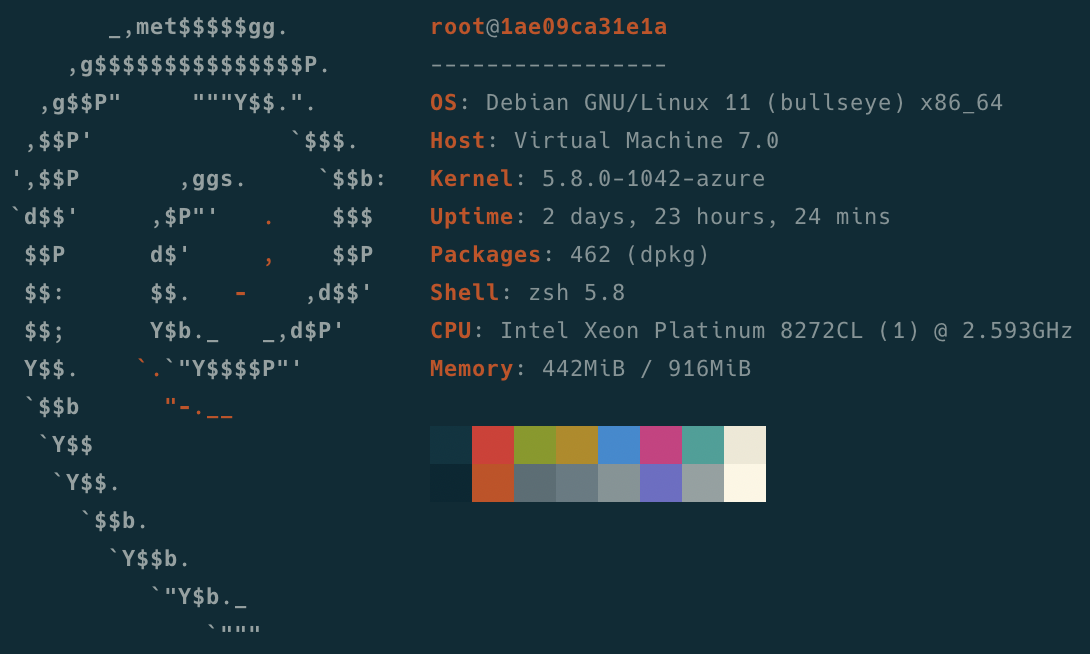
\includegraphics[width=10cm]{server_sysinfo}
        \caption{Server system information}
        \label{fig:server_sysinfo}
    \end{figure}
  }
\end{enumerate}

\section{Experimental details}\label{sec:experimental-details}
\begin{enumerate}[label=(\alph*)]
  \item {
    Experiment 1\\\\
    Request 100 read operations, the data size is 100 bytes, and the average response time is 0.40775113833000004 seconds.\\
    Request 100 write operations, the data size is 100 bytes, and the average response time is 0.4097092793800001 seconds.\\
    Request 100 modification operations, the data size is 100 bytes, and the average response time is 0.418472302340725 seconds.\\
  }
  \item {
    Experiment 2\\\\
    Request 100 write operations, the data size is 10 bytes, and the average response time is 0.4070674958099999 seconds.\\
    Request 100 write operations, the data size is 1000 bytes, and the average response time is 0.41493206457999965 seconds.\\
    Request 100 write operations, the data size is 100000 bytes, and the average response time is 0.6903830932800006 seconds.\\
  }
  \item {
    Experiment 3\\\\
    Request 100 modification operations, the data size is 100 bytes, and the average response time is 0.418472302340725 seconds.\\
    Request 100 modification operations for complex calculations, the data size is 100 bytes, and the average response time is 0.4574660183399997 seconds.\\
  }
\end{enumerate}


\section{Source code}\label{sec:source-code}
\begin{enumerate}[label=(\alph*)]
  \item {
    The GitHub repository link is \url{https://github.com/0x00000024/rpc-experiment}
  }
  \item {
    Please refer to Figure~\ref{fig:client} for the client code.
    \begin{figure}[htp]
        \centering
        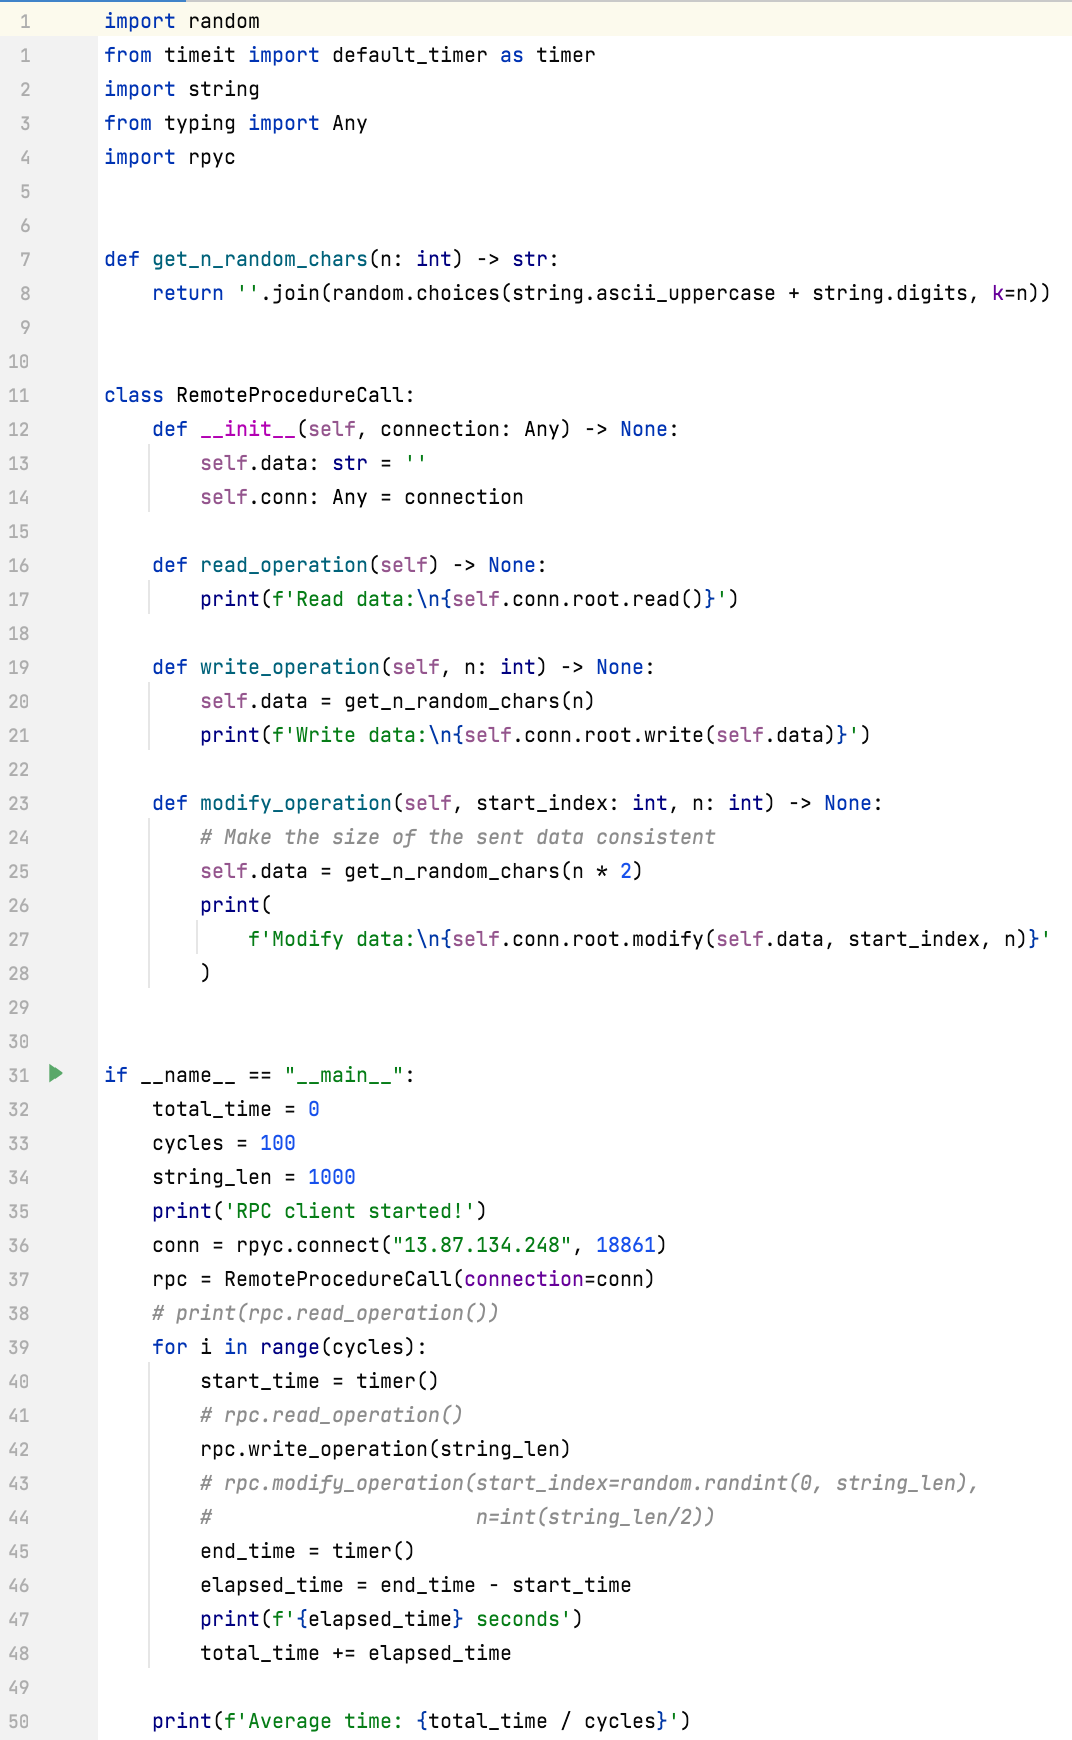
\includegraphics[width=13cm]{client}
        \caption{The source code of the client}
        \label{fig:client}
    \end{figure}
  }
  \item {
    Please refer to Figure~\ref{fig:server} for the server code.
    \begin{figure}[htp]
        \centering
        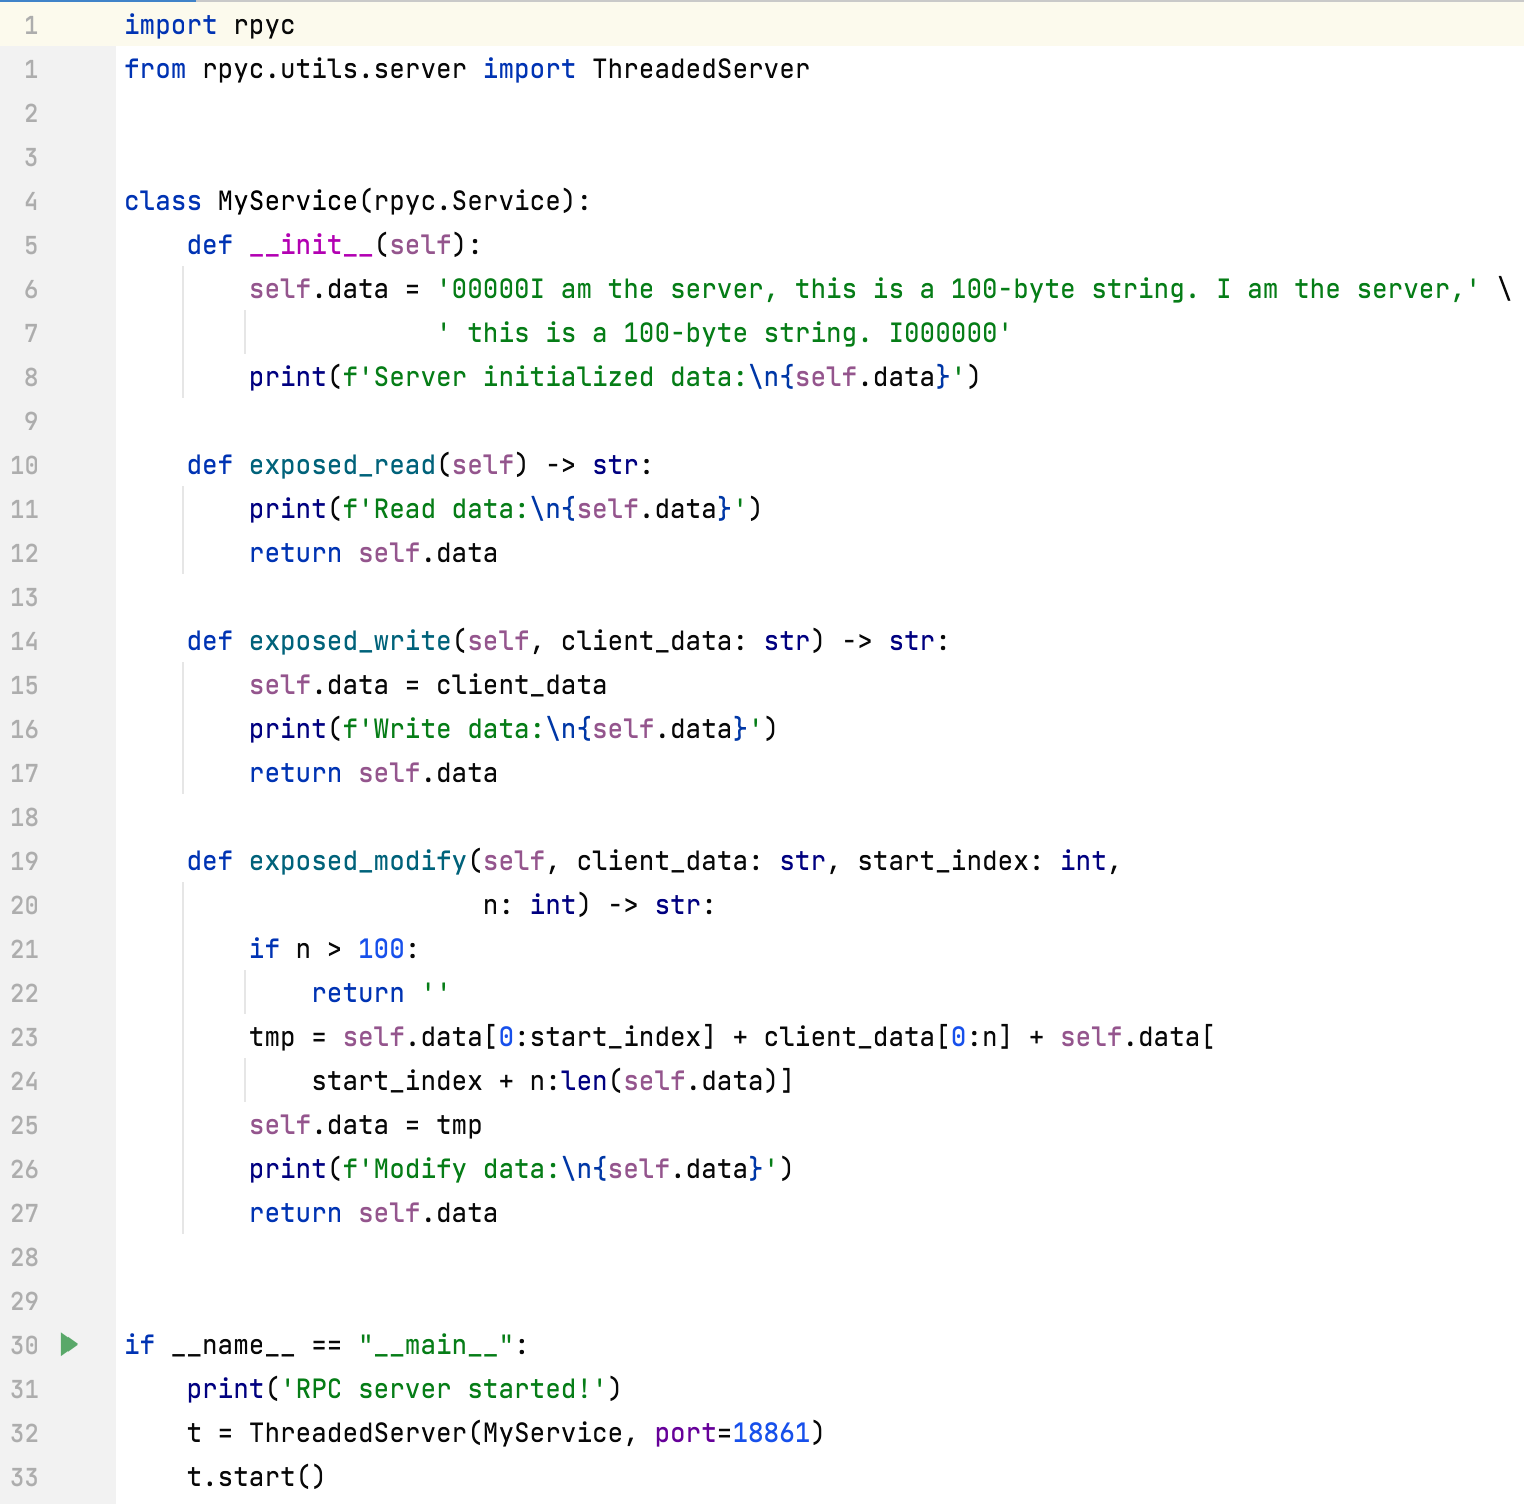
\includegraphics[width=15cm]{server}
        \caption{The source code of the server}
        \label{fig:server}
    \end{figure}
  }
\end{enumerate}


\section{Conclusion}\label{sec:conclusion}
After testing, I found that the average response time of the client calling the function in the server depends on the following two factors:
\begin{enumerate}[label=(\alph*)]
  \item How much data is transmitted in the communication process
  \item The running time of the function called remotely
\end{enumerate}


\end{document}
